The GGSW cryptosystem is a list of GLev ciphertexts. In the GGSW cryptosystem, the secret key $S$ is a list of $k$ polynomials (i.e., $S_0, S_1, ... \text{ } S_{k-1}$), and each $i$-th GLev ciphertext in the GGSW ciphertext encrypts the plaintext $S_0 \cdot M, S_1 \cdot M, ... \text{ } S_{k-1} \cdot M$, and $M$. This is visually depicted in \autoref{fig:ggsw}.


\subsection{Encryption}
\label{subsec:ggsw-enc}

\begin{tcolorbox}[title={\textbf{\tboxlabel{\ref*{subsec:ggsw-enc}} GGSW Encryption}}]
$\textsf{GGSW}_{S, \sigma}^{\beta, l}(M) = \Bigl \{ \{ \textsf{GLev}_{S, \sigma}^{\beta, l}(-S_i \cdot M)  \}_{i=0}^{k-1}, \textsf{GLev}_{S, \sigma}^{\beta, l}(M) \Bigr \} \in \mathcal{R}_{\langle n, q \rangle }^{(k+1) \cdot l \cdot (k+1)}$
\end{tcolorbox}

\begin{figure}[h!]
    \centering
  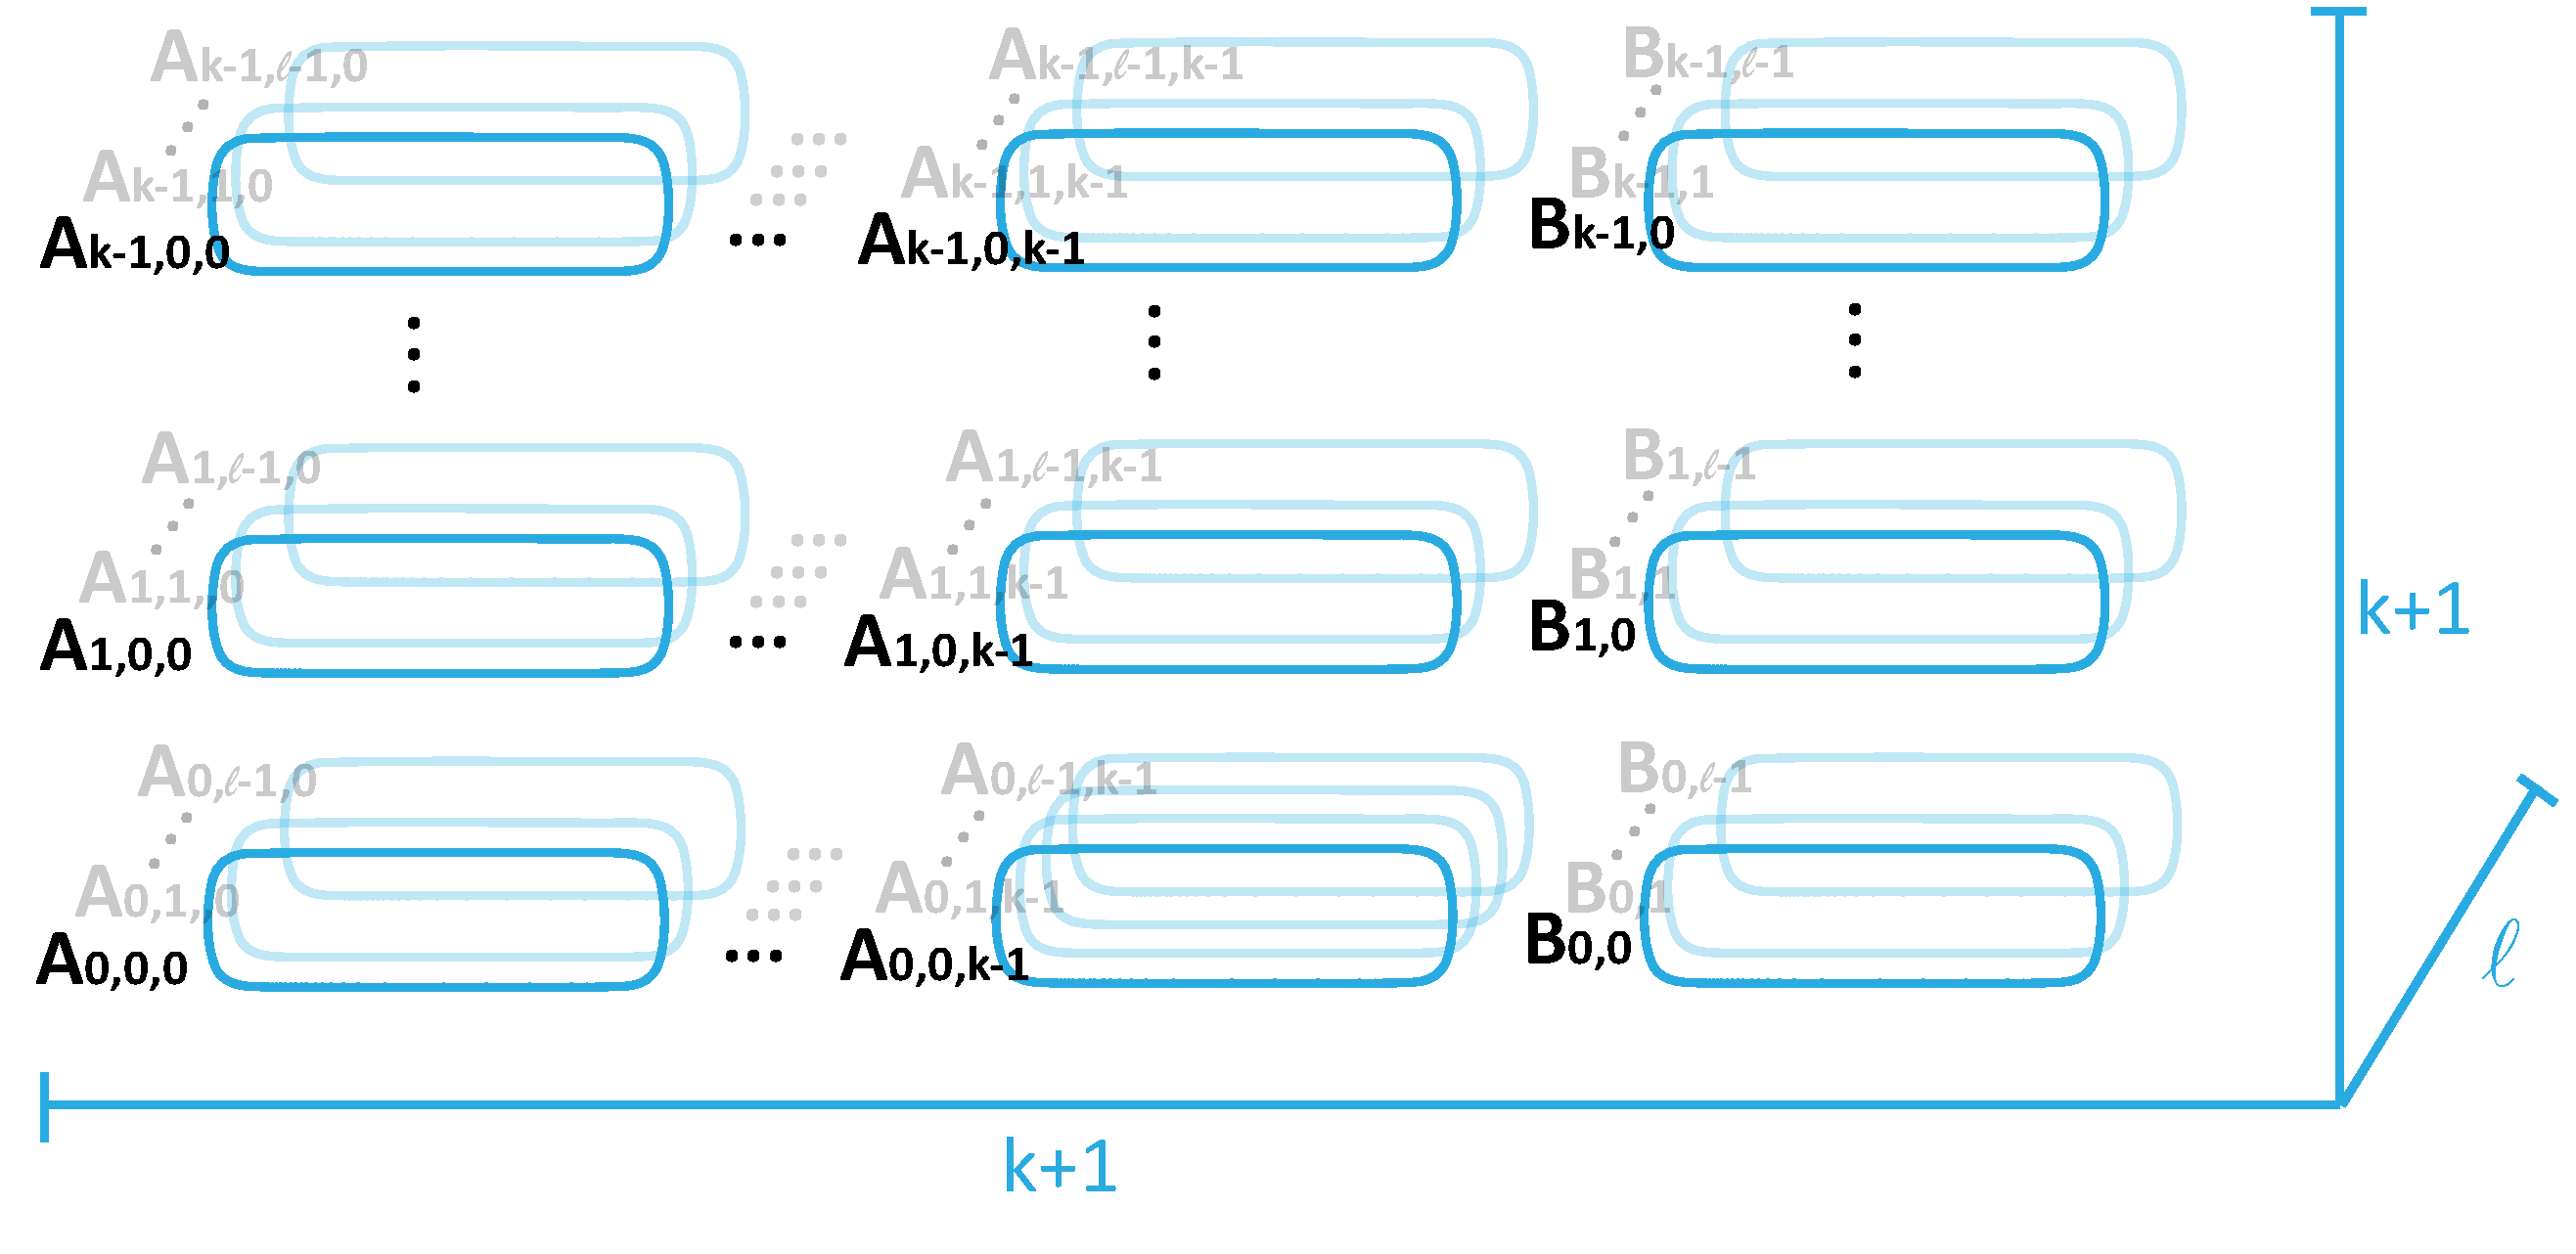
\includegraphics[width=1.0\linewidth]{figures/TFHE-fig3.pdf}
  \caption{An illustration of a GGSW ciphertext}
  \label{fig:ggsw}
\end{figure}


\subsection{Decryption}

It is sufficient to decrypt the GGSW ciphertext's any one GLev ciphertext's any one GLWE ciphertext, by using the secret $S$.



\subsection{GSW and RGSW}

GSW is GLev with $n=1$. RGSW is GLev with $k=1$.